\chapter{Testing and results}\label{chap:TestingAndResults}
The main testing of the system was preformed in the machine hall of UiA. Figure \ref{fig:testSetup} illustrates the test setup. The Husky (left side of picture) are positioned in front of a backpack, placed outside of the FOV of the lidar, (right side of picture). The test was run with and without the radars active, to see the effect the radars give the system. The test procedure consisted of first mapping the area with SLAM, by driving the Husky around manually, then the test setup would be assumed. NAV2 would be asked to drive to a location behind the backpack to test whether the Husky would crash in to the backpack or not. 

\begin{figure}[H]
    \centering
    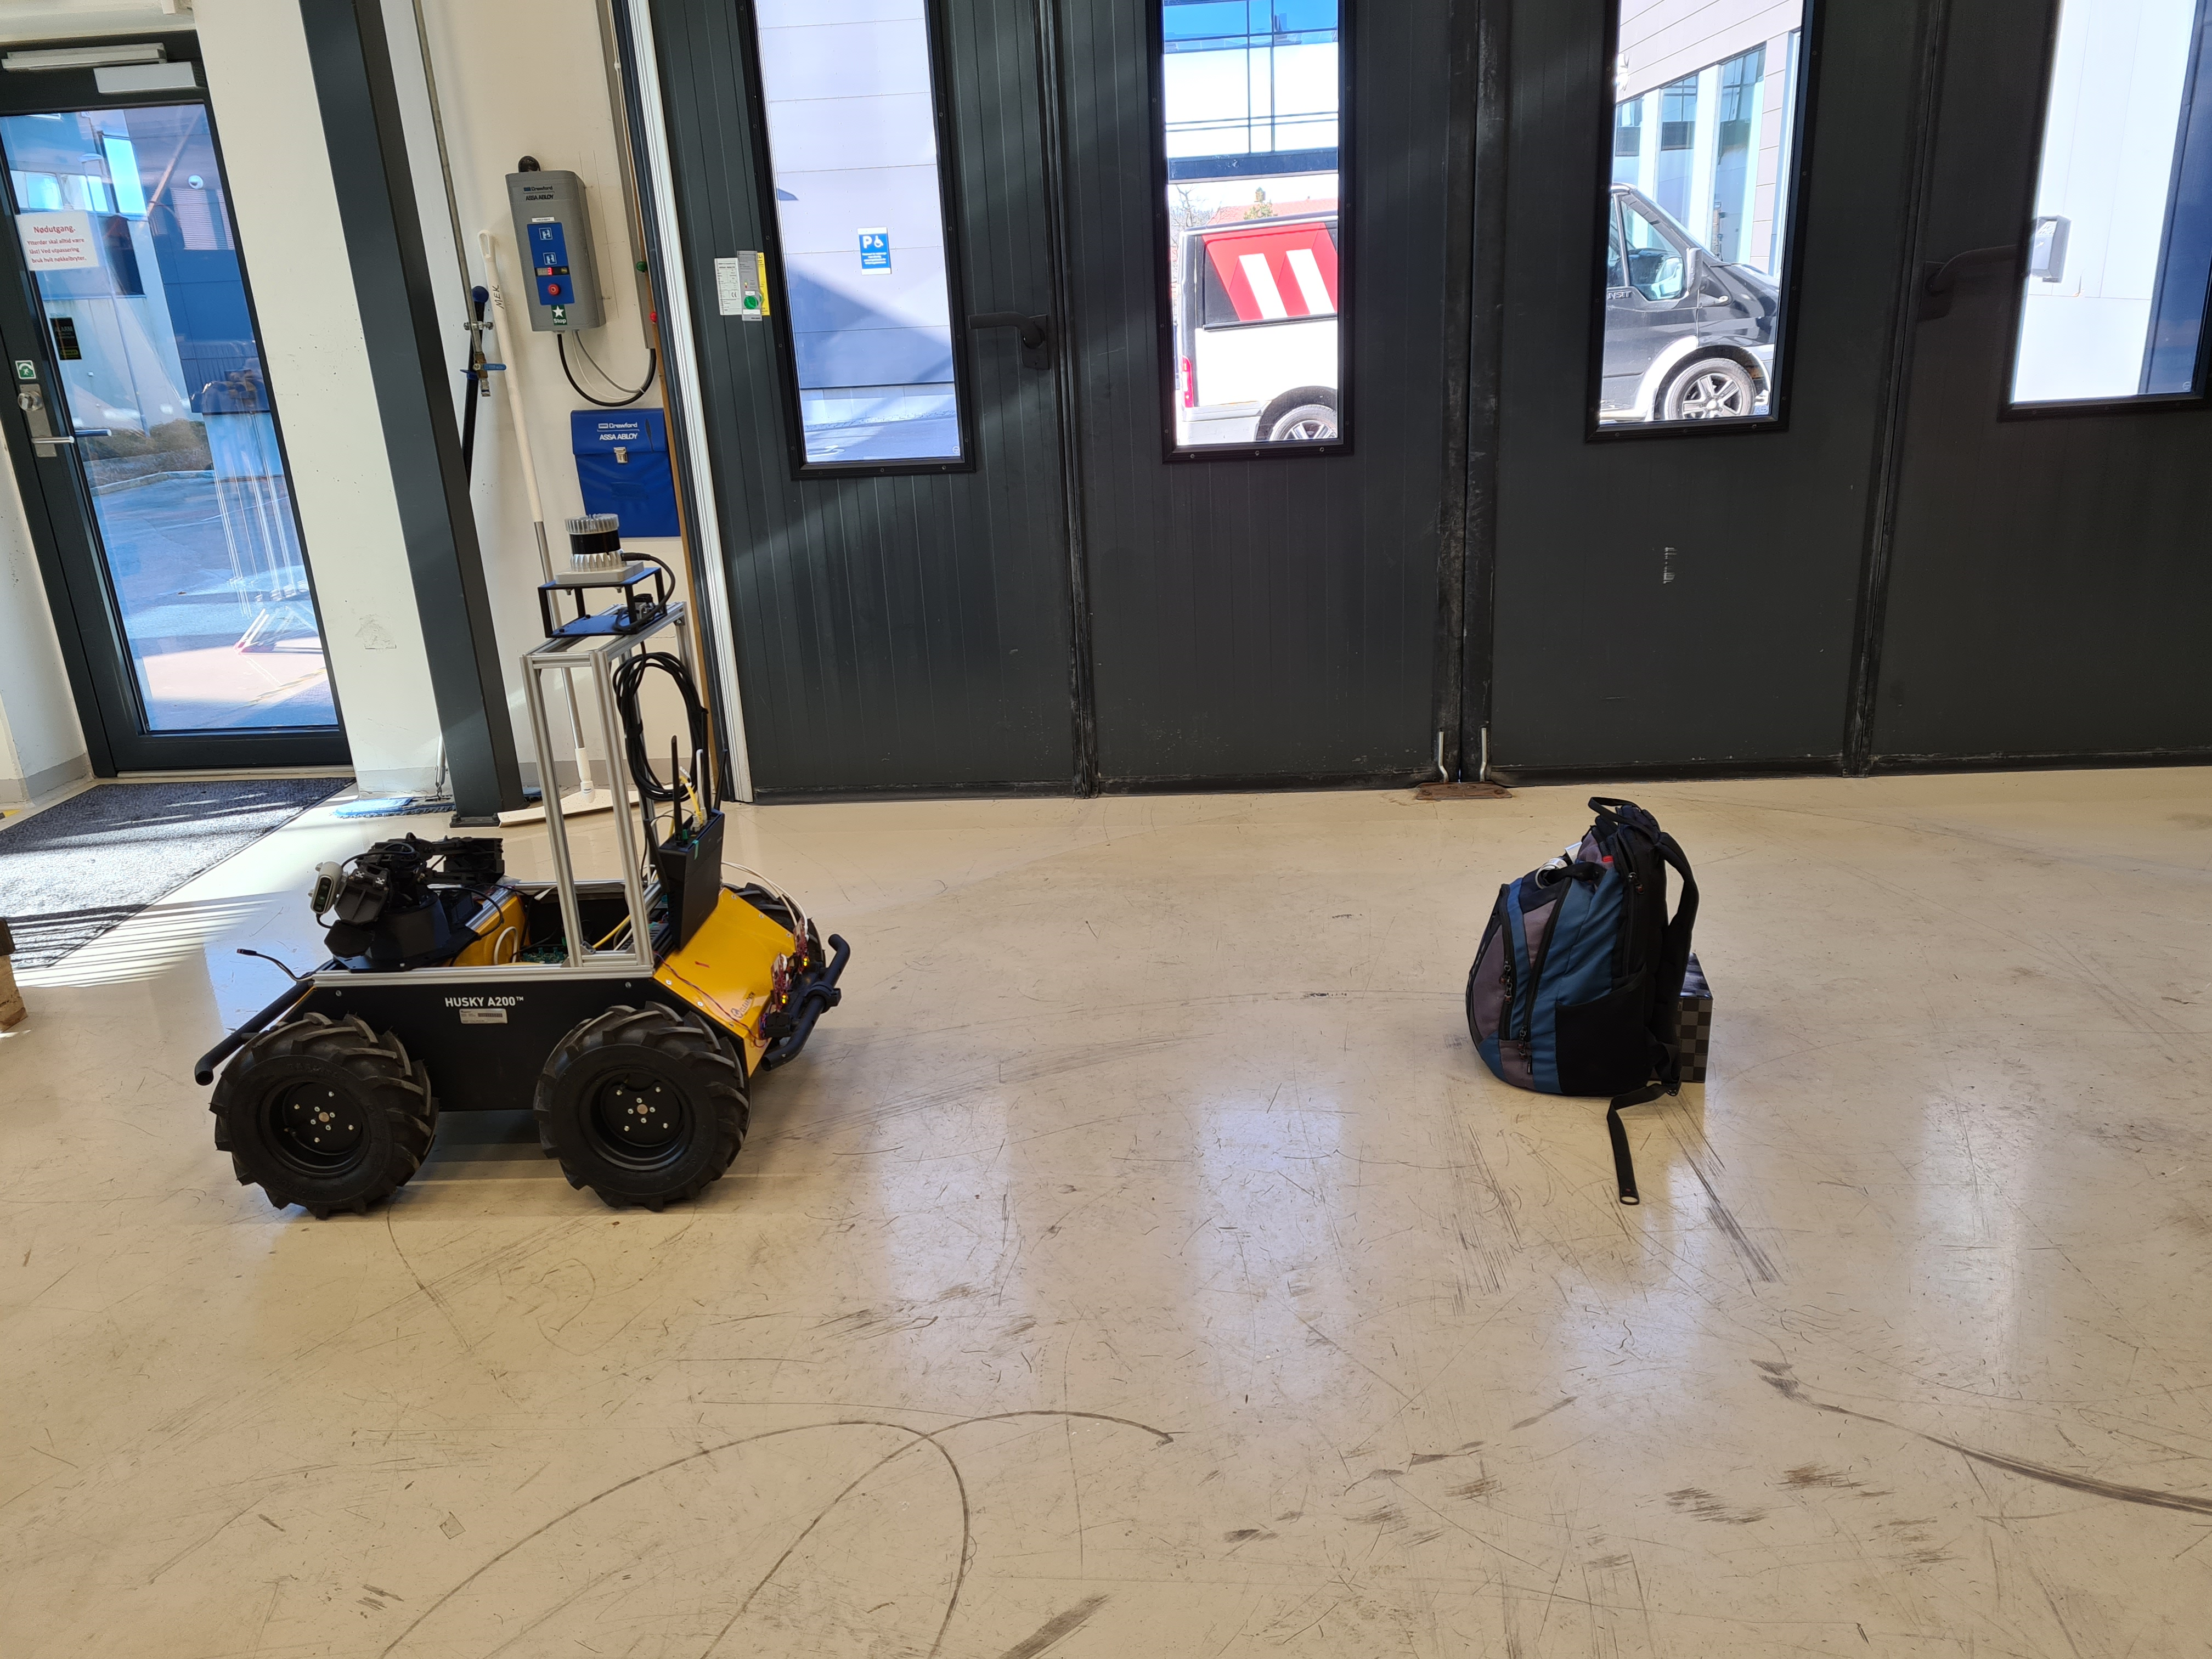
\includegraphics[width=1\textwidth]{Figures/testSetup.png}
    \caption{Test setup. Husky on left positioned towards backpack (right). The backpack is propped up by a battery (black and grey box).}
    \label{fig:testSetup}
\end{figure}

Figure \ref{fig:slamWithRadarRos2} displays the ROS2 part of the system trough a screenshot of Rviz2, this will be explained further below. Figure \ref{fig:slamWithRadarRos1} displays the ROS1 part of the system, in the form of a screenshot of Rviz. The radar mount can bee seen with two radar modules mounted to it, some distance away form the base link/base reference frame. Three colourful spheres can be viewed directly above the radar modules, these represent ranging data from the radars. More radar data/points can bee seen can be observed near the right edge of the figure (\ref{fig:slamWithRadarRos1}), at the upper half. The tree points just above the radar modules seem to be static and a product of some kind of noise or error, they are therefore "filtered" out by the \textit{flatten.launch} functionality (see \ref{subsubsec:flatten.launch}). The smaller, less colourful points (mostly orange, yellow and green) represents the 3D pointcloud of the lidar. Each square that makes up the grid seen in the figure measures $10 cm$ by $10 cm$. 

Figure \ref{fig:slamWithRadarRos2} displays the ROS2 part of the system, in the form of a screenshot of Rviz2. The husky can bee seen near the middle of the figure, sitting on top a light grey surface with black squares (mostly) separating the light grey area from a dark grey area. These grey and black areas represents the map produced by SLAM. Light grey represents unobstructed areas where the Husky can navigate, black are occupied areas and dark grey areas are unknown/unobserved areas. The difficult to spot, white points near the black areas represent the merged range data of the ROS1 system (two radar modules and a lidar). Figure \ref{fig:radarAndLidarPointsInRos2} better illustrates the merged range data. Each square that makes up the grid seen in the figure measures $1 m$ by $1 m$.

\begin{figure}[H]
    \centering
    \begin{minipage}[b]{0.49\textwidth}
        \includegraphics[width=\textwidth,trim={7cm 4cm 25cm 7cm},clip]{Figures/slamWithRadar.png}
        \caption{Zoomed in view of Rviz2 showing the Husky in a map produced by SLAM. Small dots around the black areas represent merged range data from ROS1 (seen in figure \ref{fig:slamWithRadarRos1}). Based on figure \ref{fig:slamWithRadar}.}
        \label{fig:slamWithRadarRos2}
    \end{minipage}
    %\hfill
    \begin{minipage}[b]{0.49\textwidth}
        \includegraphics[width=\textwidth,trim={25cm 7cm 7cm 4cm},clip]{Figures/slamWithRadar.png}
        \caption{Zoomed in view of Rviz displaying the ranging data from the radars and the lidar. The bigger more colourful points are produced by the radars, the rest are from the lidar. The radar mount with two radar modules mounted are also visible. Based on figure \ref{fig:slamWithRadar}.}
        \label{fig:slamWithRadarRos1}
    \end{minipage}
\end{figure}

\begin{figure}[H]
    \centering
    \includegraphics[width=0.8\textwidth]{Figures/radarAndLidarPointsInRos2.png}
    \caption{Better view of points representing the ranging data from ROS1, simmilar to the points in figure \ref{fig:slamWithRadarRos2}}
    \label{fig:radarAndLidarPointsInRos2}
\end{figure}

\section{Test with lidar (without radar)}
Figure \ref{fig:slamWithoutRadar} illustrate the SLAM-process of the test, but only based on range data from the lidar. The figure has similar properties to figure \ref{fig:slamWithRadarRos2} and \ref{fig:slamWithRadarRos1}, but the radar modules, and their data, is missing from Rviz (right side). The test uses a modified version of the algorithm, described in chapter \ref{sec:Algorithm}, where step 2.a, 2.c and 3 is not used, but the rest are.

\begin{figure}[H]
    \centering
    \includegraphics[width=\textwidth]{Figures/slamWithoutRadar.png}
    \caption{{View of ROS2 system (left) and ROS1 system (right) while SLAM runs without the radars. See figure \ref{fig:slamWithRadarRos1} and \ref{fig:slamWithRadarRos2} for a better understanding of figure.}}
    \label{fig:slamWithoutRadar}
\end{figure}

The testing position (displayed in figure \ref{fig:testSetup}) was assumed after a map was created. The test was den conducted as explained above. Figure \ref{fig:crashWithoutRadar} shows the aftermath of the test, where the Husky is standing on top of the backpack, after failing to detect and avoid it. Purple, pink and cyan areas displayed on the left side of the figure indicates detected objects, or areas to avoid. The colourful areas are part of the cost map.

\begin{figure}[H]
    \centering
    \includegraphics[width=\textwidth]{Figures/crashWithoutRadar.png}
    \caption{Failed collision avoidance test. The husky is standing on top of the backpack. Purple, pink and cyan areas indicating detected objects (cost map).}
    \label{fig:crashWithoutRadar}
\end{figure}

Figure \ref{fig:preCrashWithoutRadar} was captured just moments before \ref{fig:crashWithoutRadar}, where the backpack is not visible on the cost map. 

\begin{figure}[H]
    \centering
    \includegraphics[width=\textwidth]{Figures/preCrashWithoutRadar.png}
    \caption{Failed collision avoidance test. Moments before failure. See figure \ref{fig:crashWithoutRadar} for collision.}
    \label{fig:preCrashWithoutRadar}
\end{figure}

\section{Test with radar and lidar}
Figure \ref{fig:slamWithRadar} displays the SLAM part of the test, but now with the radars. The test uses all of the steps of the algorithm described in chapter \ref{sec:Algorithm}.

\begin{figure}[H]
    \centering
    \includegraphics[width=\textwidth]{Figures/slamWithRadar.png}
    \caption{View of ROS2 system (left) and ROS1 system (right) while SLAM runs with the radars and the lidar. See figure \ref{fig:slamWithRadarRos1} and \ref{fig:slamWithRadarRos2} for more detail.}
    \label{fig:slamWithRadar}
\end{figure}

The test procedure was conducted similarly to above with the new map and radars activated. Figure \ref{fig:crashWithRadar} shows the aftermath of the test, where the Husky has stopped in front of the backpack. One can barley make out the colourful spheres that represents the radars' detection of the backpack.

\begin{figure}[H]
    \centering
    \includegraphics[width=\textwidth]{Figures/crashWithRadar.png}
    \caption{Husky standing still after stopping in front detected object, see figure \ref{fig:crashWithoutRadar}, \ref{fig:slamWithRadarRos2} and \ref{fig:slamWithRadarRos1} for better understanding}
    \label{fig:crashWithRadar}
\end{figure}


